% Provenance (never printed): see sources/outline_sources.md (Year 1: gravity and its
% measurement, normal gravity; isostasy, Airy and Pratt; free-air and Bouguer anomalies;
% the geoid). Curves from figdata/bachelor-1/hypsometry.py and gravity_profiles.py;
% exercise and problem values in the Book 3 scratch calculator calc/ch11.py.
\chapter{Isostasie et anomalies de pesanteur}\label{ch:b1:isostasy-gravity}

Dans les années 1840, les arpenteurs qui mesuraient un arc de méridien à travers
le nord de l'Inde se heurtèrent à un désaccord qu'ils ne pouvaient imputer à
leurs instruments. Entre deux stations distantes d'environ 370 milles, Kaliana au
pied de l'Himalaya et Kalianpur loin au sud, la différence de \omterm{def:b1:spherical-astronomy:geographic}{latitude} trouvée par
triangulation dépassait de 5.236 secondes d'arc celle trouvée par les étoiles.
Le coupable évident était la montagne~: son attraction tire le fil à plomb vers
le nord, et les astronomes réglaient leurs instruments sur le fil à plomb. En 1855,
John Henry Pratt calcula l'attraction de l'Himalaya et des plateaux qui le
prolongent et trouva qu'elle aurait dû produire un désaccord de 15.885 secondes,
plus de trois fois ce qu'on observait. Les montagnes attiraient bien moins que leur
masse visible ne l'exigeait. La même année, George Airy répondit que la \omterm{def:b1:layered-earth:layers}{croûte}
flotte sur une couche plus dense comme un radeau de rondins sur l'eau, si bien
qu'un terrain élevé a une profonde racine de roche légère~; Pratt proposa plus
tard une autre réponse, une roche rendue plus légère par dilatation sous les
montagnes. Les deux sont encore enseignées~: les montagnes reposent sur de la
roche légère qui compense leur masse. Ce chapitre traduit cette idée en
nombres, et montre comment la pesanteur, mesurée au millionième de sa valeur,
révèle les masses cachées sous le relief.
% ledger: pratt:himalaya, airy:1855, pratt:1871

\begin{recall}
La loi de la gravitation de Newton donne le champ $g = GM/r^2$ à l'extérieur d'une
masse sphérique $M$~; le champ dérive d'un potentiel gravitationnel, et une
surface équipotentielle est partout perpendiculaire au champ (physique). Dans un
fluide au repos la pression croît avec la profondeur selon $\mathrm dp/\mathrm dz = \rho g$,
et un corps flottant déplace son propre poids de fluide (physique, volume de première
année). Sous la \omterm{def:b1:layered-earth:lithosphere}{lithosphère} l'\omterm{def:b1:layered-earth:lithosphere}{asthénosphère} s'écoule sur de longues durées~; la
\omterm{def:b1:layered-earth:layers}{croûte} est plus légère que le \omterm{def:b1:layered-earth:layers}{manteau} qui la porte (\cref{ch:b1:layered-earth}~;
livre~2, année~11).
\end{recall}

\section{La pesanteur et sa mesure}

L'accélération de la pesanteur à la surface de la Terre est voisine de
\qty{9.8}{m.s^{-2}}, et les variations qui intéressent les géologues sont un
million de fois plus petites. On les compte dans une unité de l'ancien système
centimètre--gramme, le gal~: $\qty{1}{Gal} = \qty{1}{cm.s^{-2}} = \qty{0.01}{m.s^{-2}}$, de sorte
que
\[
  \qty{1}{\milli\gal} = \qty{e-5}{m.s^{-2}} \approx \num{e-6}\,g .
\]
% ledger: nist:gal
Un instrument de terrain résout quelques millièmes de milligal~; les anomalies
étudiées dans ce chapitre vont d'une fraction de milligal au-dessus d'un
gisement enfoui à quelques centaines de milligals au-dessus d'une chaîne de
montagnes.

Même sur une Terre sans relief, la pesanteur ne serait pas partout la même. La
Terre tourne, si bien que ce que sentent un fil à plomb ou un gravimètre est la
somme de l'attraction gravitationnelle et de l'effet centrifuge de la rotation~;
et la Terre est aplatie, si bien que les pôles sont plus près de son centre que
l'équateur. Les deux effets rendent la pesanteur plus faible à l'équateur qu'aux
pôles. Le géologue compare chaque mesure à une référence lisse qui les contient.

\begin{definition}[Pesanteur normale]\label{def:b1:isostasy-gravity:normal-gravity}
La \emph{pesanteur normale}\index{pesanteur normale} $\gamma$ est la pesanteur d'une
Terre modèle~: un ellipsoïde de révolution de la masse et de la rotation de la Terre,
choisi de sorte que sa surface soit une équipotentielle de sa propre pesanteur
(gravitation plus effet centrifuge). Sur cette surface, la pesanteur normale ne
dépend que de la \omterm{def:b1:spherical-astronomy:geographic}{latitude}.
\end{definition}

L'ellipsoïde lui-même, son aplatissement et la façon dont ses paramètres sont
ajustés à la Terre réelle sont étudiés au livre~5. Ici nous n'avons besoin que de
sa pesanteur.

\begin{proposition}[La formule de la pesanteur normale]\label{prop:b1:isostasy-gravity:normal-formula}
Sur l'ellipsoïde de référence adopté en 1980, la \omterm{def:b1:isostasy-gravity:normal-gravity}{pesanteur normale} à la \omterm{def:b1:spherical-astronomy:geographic}{latitude}
géographique $\varphi$ est, sous sa forme usuelle en série,
\[
  \gamma(\varphi) = \qty{9.780327}{m.s^{-2}}\,\bigl(1 + 0.0053024\sin^2\varphi
  - 0.0000058\sin^2 2\varphi\bigr).
\]
\end{proposition}
\admitted
% ledger: moritz:grs80

Elle donne \qty{9.780327}{m.s^{-2}} à l'équateur, \qty{9.806200}{m.s^{-2}} à
\ang{45} et \qty{9.832186}{m.s^{-2}} aux pôles~: une différence de
\qty{5186}{\milli\gal} de l'équateur au pôle. La rotation à elle seule en explique
l'essentiel. Avec le jour sidéral de \qty{23.9345}{h}, la vitesse angulaire est
$\omega = 2\pi/\qty{86164}{s} = \qty{7.292e-5}{rad.s^{-1}}$, et l'accélération
centrifuge à l'équateur, $\omega^2 a$ avec $a = \qty{6378.137}{km}$, est de
\qty{0.0339}{m.s^{-2}}, soit \qty{3392}{\milli\gal}~; l'aplatissement fournit le
reste (\cref{exo:b1:isostasy-gravity:2}).
% ledger: earth:Trot, earth:Req, earth:geq, earth:gpole

La pesanteur se mesure de deux façons. Un gravimètre \emph{absolu} lâche une masse
d'épreuve dans une chambre à vide et suit sa chute libre par un interféromètre
laser, cadencé par une horloge atomique~: l'accélération sort directement de la
distance et du temps. Un gravimètre \emph{relatif} est une masse suspendue à un
ressort, dont l'allongement change avec la pesanteur~; il est léger et rapide,
mais il ne donne que des différences entre lieux, et il dérive, si bien qu'un
levé revient à une station de base dont la pesanteur est connue. Les meilleurs
instruments absolus sont exacts à environ un microgal, un milliardième de $g$.
% ledger: ngs:absolute-gravity

\begin{inthefield}[Un levé gravimétrique à terre]
\begin{minipage}[t]{0.55\linewidth}\vspace{0pt}
Un levé gravimétrique est une lente marche de station en station. À chacune, le
géophysicien pose le gravimètre relatif sur son trépied, le cale, attend que le
ressort se stabilise et fait plusieurs lectures~; un récepteur de positionnement
par satellite à côté de lui enregistre la position et la hauteur de la station.
Toutes les quelques heures l'équipe retourne à la station de base, afin que la
dérive du ressort puisse être mesurée et retirée. La hauteur compte autant que la
pesanteur~: comme le montre la section suivante, la pesanteur diminue de
\qty{0.3086}{\milli\gal} par mètre de hauteur, si bien qu'une hauteur fausse de
\qty{1}{cm} gâte la lecture de \qty{3}{\micro\gal}. % ledger: usgs73:reduction
\end{minipage}\hfill
\begin{minipage}[t]{0.42\linewidth}\vspace{0pt}
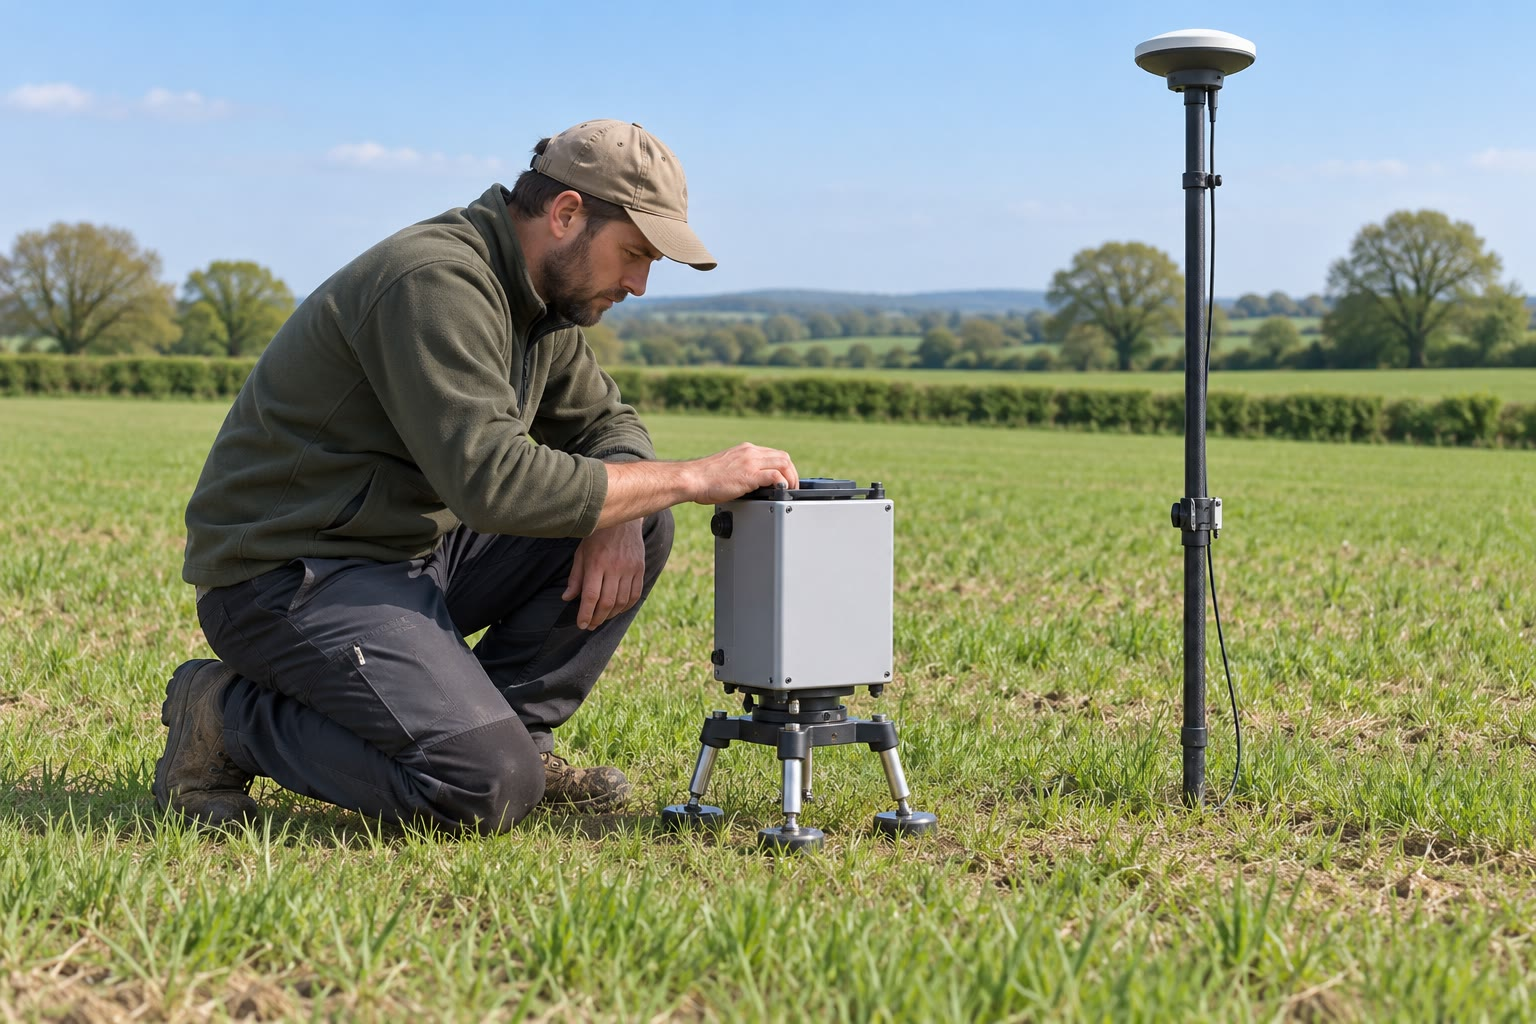
\includegraphics[width=\linewidth]{images/book3/ai/b1-gravity-survey.jpg}

{\scriptsize Un gravimètre de terrain sur son trépied, avec une antenne de
positionnement par satellite à côté (illustration générée par IA).}
\end{minipage}
\end{inthefield}

\section{L'isostasie}

La compensation qu'Airy et Pratt imaginaient pour l'Himalaya est un cas d'un état
général des couches externes de la Terre.

\begin{definition}[Isostasie~; profondeur de compensation]\label{def:b1:isostasy-gravity:isostasy}
Une région est en \emph{isostasie}\index{isostasie}, ou équilibre isostatique, quand
il existe une profondeur, la \emph{profondeur de compensation}\index{profondeur de compensation},
où la pression est la même en tout point de la surface horizontale,
quel que soit le relief au-dessus. Au-dessous de la profondeur de compensation les
roches se comportent comme un fluide au repos~; au-dessus, les colonnes de \omterm{def:b1:layered-earth:layers}{croûte} et
de \omterm{def:b1:layered-earth:layers}{manteau} flottent sur elles.
\end{definition}

\begin{proposition}[Masses égales au-dessus de la profondeur de compensation]\label{prop:b1:isostasy-gravity:equal-mass}
Si la pesanteur $g$ est la même le long de toutes les colonnes, une région est en
\omterm{def:b1:isostasy-gravity:isostasy}{isostasie} avec la \omterm{def:b1:isostasy-gravity:isostasy}{profondeur de compensation} $z_c$ si et seulement si chaque colonne
verticale de section unité, de la surface jusqu'à $z_c$, contient la même masse.
\end{proposition}

\begin{proof}
Dans chaque colonne les roches sont en équilibre hydrostatique, de sorte que
$\mathrm dp/\mathrm dz = \rho(z)\,g$, la profondeur $z$ étant comptée vers le bas. La
pression à la surface est atmosphérique, la même partout (et négligeable).
En intégrant de la surface $z_s$ de la colonne jusqu'à $z_c$ on obtient
\[
  p(z_c) = p_0 + g\int_{z_s}^{z_c}\rho(z)\,\mathrm dz ,
\]
où l'intégrale est la masse de la colonne par unité d'aire. Les pressions en
$z_c$ sont égales si et seulement si ces masses le sont.
\end{proof}

Deux manières simples de répartir les masses donnent les deux modèles classiques
(figure ci-dessous).

\begin{proposition}[Isostasie d'Airy]\label{prop:b1:isostasy-gravity:airy}
Soit une \omterm{def:b1:layered-earth:layers}{croûte} de masse volumique uniforme $\rho_c$ et d'épaisseur $H$ là où sa
surface est au niveau de la mer, sur un \omterm{def:b1:layered-earth:layers}{manteau} de masse volumique $\rho_m > \rho_c$.
À l'équilibre isostatique~:
\begin{enumerate}
  \item là où la surface se tient à une hauteur $h$ au-dessus du niveau de la mer,
        la \omterm{def:b1:layered-earth:layers}{croûte} a une racine de profondeur $r = h\,\rho_c/(\rho_m - \rho_c)$ sous
        la \omterm{def:b1:layered-earth:layers}{croûte} normale, et une épaisseur $H + h + r$~;
  \item là où la surface se trouve à une profondeur $d$ sous le niveau de la mer,
        sous une eau de masse volumique $\rho_w$, la \omterm{def:b1:layered-earth:layers}{croûte} a une anti-racine~: sa
        base est relevée de
        $r' = d\,(\rho_c - \rho_w)/(\rho_m - \rho_c)$, et son épaisseur est
        $H - d - r'$.
\end{enumerate}
C'est l'\emph{isostasie d'Airy}\index{isostasie d'Airy}~: compensation par des
changements d'épaisseur à masse volumique constante.
\end{proposition}

\begin{proof}
Prenons la \omterm{def:b1:isostasy-gravity:isostasy}{profondeur de compensation} juste sous la racine la plus profonde, et
comparons chaque colonne à la colonne normale. (1) La colonne haute a de la \omterm{def:b1:layered-earth:layers}{croûte} à
la place du \omterm{def:b1:layered-earth:layers}{manteau} sur la profondeur $r$, et de la \omterm{def:b1:layered-earth:layers}{croûte} sur la hauteur $h$ là où
la colonne normale n'a rien~: l'égalité des masses exige $\rho_c(h + r) = \rho_m r$,
c'est-à-dire $r(\rho_m - \rho_c) = \rho_c h$. (2) La colonne basse a de l'eau à la
place de la \omterm{def:b1:layered-earth:layers}{croûte} sur la profondeur $d$, et du \omterm{def:b1:layered-earth:layers}{manteau} à la place de la \omterm{def:b1:layered-earth:layers}{croûte} sur
$r'$~: l'égalité des masses exige
$\rho_w d + \rho_m r' = \rho_c(d + r')$, c'est-à-dire $r'(\rho_m - \rho_c) =
d(\rho_c - \rho_w)$.
\end{proof}

\begin{proposition}[Isostasie de Pratt]\label{prop:b1:isostasy-gravity:pratt}
Soit des colonnes qui se terminent toutes à la même \omterm{def:b1:isostasy-gravity:isostasy}{profondeur de compensation} $D$
sous le niveau de la mer, avec une masse volumique uniforme dans chaque colonne,
$\rho_0$ là où la surface est au niveau de la mer. À l'équilibre isostatique une
colonne dont la surface se tient à une hauteur $h$ a la masse volumique
\[
  \rho(h) = \rho_0\,\frac{D}{D + h},
\]
et une colonne sous une profondeur $d$ d'eau a la masse volumique
$\rho = (\rho_0 D - \rho_w d)/(D - d)$. C'est l'\emph{isostasie de
Pratt}\index{isostasie de Pratt}~: compensation par des changements de masse
volumique à profondeur constante.
\end{proposition}

\begin{proof}
Masses égales au-dessus de $D$~: $\rho(h)(D + h) = \rho_0 D$ pour la colonne haute, et
$\rho_w d + \rho(D - d) = \rho_0 D$ pour la colonne basse.
\end{proof}

Avec $\rho_c = \qty{2700}{kg.m^{-3}}$ et $\rho_m = \qty{3300}{kg.m^{-3}}$, la
racine d'Airy est $h\times2700/600 = 4.5\,h$~: une chaîne haute de \qty{2}{km} a une
racine de \qty{9}{km}, un plateau haut de \qty{4}{km} une de \qty{18}{km}. Dans le
modèle de Pratt avec $D = \qty{100}{km}$ et $\rho_0 = \qty{2700}{kg.m^{-3}}$, les
deux mêmes colonnes ont les masses volumiques 2647 et \qty{2596}{kg.m^{-3}}, plus
légères de deux et quatre pour cent. Les deux modèles équilibrent les mêmes masses~;
ils diffèrent par l'endroit où se trouve la roche légère, et c'est ce que la
sismologie peut voir~: Airy prédit un \omterm{def:b1:layered-earth:discontinuity}{Moho} qui s'approfondit sous les montagnes,
Pratt un \omterm{def:b1:layered-earth:discontinuity}{Moho} plat.

\begin{omfigure}
\begin{tikzpicture}[x=0.55cm, y=0.05cm, font=\scriptsize]
% columns computed in calc/ch11.py: Airy roots 9 and 18 km, Pratt densities 2647 and 2596 kg/m3;
% heights above sea level drawn five times larger than depths
\begin{scope}
  \node[font=\small] at (4.5,30) {(a) Airy};
  \fill[omLithGranite!45] (0,0) rectangle (3,-35);
  \fill[omLithGranite!45] (3,10) rectangle (6,-44);
  \fill[omLithGranite!45] (6,20) rectangle (9,-53);
  \fill[omLithPeridotite!45] (0,-35) rectangle (3,-60);
  \fill[omLithPeridotite!45] (3,-44) rectangle (6,-60);
  \fill[omLithPeridotite!45] (6,-53) rectangle (9,-60);
  \draw (0,-60) -- (0,0) -- (3,0) -- (3,10) -- (6,10) -- (6,20) -- (9,20) -- (9,-60);
  \draw (3,0) -- (3,-60) (6,10) -- (6,-60);
  \draw[thick] (0,-35) -- (3,-35) -- (3,-44) -- (6,-44) -- (6,-53) -- (9,-53);
  \draw[densely dashed] (-0.3,-60) -- (9.3,-60);
  \draw[black!50, densely dotted] (-0.3,0) -- (0,0);
  \node[anchor=east] at (-0.3,0) {niveau de la mer};
  \node[anchor=east] at (-0.3,-35) {35};
  \node[anchor=east] at (-0.3,-60) {60 km};
  \node at (1.5,-17) {2700}; \node at (4.5,-20) {2700}; \node at (7.5,-24) {2700};
  \node at (1.5,-50) {3300};
  \node[anchor=south] at (1.5,0) {$h = 0$};
  \node[anchor=south] at (4.5,10) {$h = 2$};
  \node[anchor=south] at (7.5,20) {$h = 4$};
  \draw[black!45, densely dotted] (3,-35) -- (9,-35);
  \node at (4.5,-39.5) {racine 9};
  \node at (7.5,-44) {racine 18};
\end{scope}
\begin{scope}[xshift=7.9cm]
  \node[font=\small] at (4.5,30) {(b) Pratt};
  \fill[omLithGranite!45] (0,0) rectangle (3,-100);
  \fill[omLithGranite!36] (3,10) rectangle (6,-100);
  \fill[omLithGranite!27] (6,20) rectangle (9,-100);
  \draw (0,-100) -- (0,0) -- (3,0) -- (3,10) -- (6,10) -- (6,20) -- (9,20) -- (9,-100);
  \draw (3,0) -- (3,-100) (6,10) -- (6,-100);
  \draw[densely dashed] (-0.3,-100) -- (9.3,-100);
  \draw[black!50, densely dotted] (-0.3,0) -- (0,0);
  \node[anchor=east] at (-0.3,0) {niveau de la mer};
  \node[anchor=east] at (-0.3,-100) {$D = 100$ km};
  \node at (1.5,-50) {2700}; \node at (4.5,-50) {2647}; \node at (7.5,-50) {2596};
  \node[anchor=south] at (1.5,0) {$h = 0$};
  \node[anchor=south] at (4.5,10) {$h = 2$};
  \node[anchor=south] at (7.5,20) {$h = 4$};
\end{scope}
\end{tikzpicture}

\par\smallskip{\small Les deux modèles classiques d'\omterm{def:b1:isostasy-gravity:isostasy}{isostasie}, pour trois colonnes
s'élevant à 0, 2 et \qty{4}{km} au-dessus du niveau de la mer (hauteurs exagérées
cinq fois par rapport aux profondeurs~; masses volumiques en \unit{kg.m^{-3}}).
(a) Airy~: une seule masse volumique de \omterm{def:b1:layered-earth:layers}{croûte}, une racine égale à 4.5 fois la
hauteur. (b) Pratt~: une seule \omterm{def:b1:isostasy-gravity:isostasy}{profondeur de compensation}, des colonnes plus légères
sous le terrain plus élevé. Chaque colonne porte la même masse par unité d'aire
au-dessus de la \omterm{def:b1:isostasy-gravity:isostasy}{profondeur de compensation} en tirets.}
\label{fig:b1:isostasy-gravity:models}
\end{omfigure}

L'\omterm{def:b1:isostasy-gravity:isostasy}{isostasie} est un énoncé sur de vastes régions et de longues durées.
L'\omterm{def:b1:layered-earth:lithosphere}{asthénosphère} ne cède qu'à des charges qui persistent des milliers d'années, et la
\omterm{def:b1:layered-earth:lithosphere}{lithosphère} au-dessus d'elle est assez rigide pour étaler une charge étroite sur
une large région en fléchissant, comme une planche porte un poids~: un volcan isolé
n'a pas besoin d'être compensé sous lui-même~; cette flexion de la \omterm{def:b1:layered-earth:lithosphere}{lithosphère} est
étudiée au livre~5. Sous les grandes chaînes de montagnes la \omterm{def:b1:layered-earth:layers}{croûte} est bien plus
épaisse que sa moyenne continentale d'environ \qty{30}{km}~: l'image d'Airy, des
racines de \omterm{def:b1:layered-earth:layers}{croûte} légère, est la plus proche pour les chaînes de montagnes. Celle de
Pratt, de la roche plus légère à profondeur constante, explique les dorsales
médio-océaniques, qui se dressent haut au-dessus d'un \omterm{def:b1:layered-earth:layers}{manteau} supérieur rendu plus
léger par sa température plus élevée.
% ledger: usgs:crust-thickness

\subsection*{Les deux niveaux de la Terre}

L'\omterm{def:b1:isostasy-gravity:isostasy}{isostasie} organise le relief de toute la planète. Sa répartition est résumée par
une seule courbe.

\begin{definition}[Courbe hypsométrique]\label{def:b1:isostasy-gravity:hypsometry}
La \emph{courbe hypsométrique}\index{courbe hypsometrique@courbe hypsométrique} d'une planète donne, pour chaque
fraction $f$ de sa surface, l'altitude $z(f)$ dépassée par exactement cette
fraction. C'est la distribution cumulative de l'altitude, lue à partir du haut.
\end{definition}

Pour la tracer à partir d'un modèle d'altitude en grille, chaque cellule doit être
pondérée par son aire. Sur une grille d'un degré en \omterm{def:b1:spherical-astronomy:geographic}{latitude} et en \omterm{def:b1:spherical-astronomy:geographic}{longitude}, la
cellule comprise entre les \omterm{def:b1:spherical-astronomy:geographic}{latitudes} $\varphi_1$ et $\varphi_2$ a l'aire
$R^2\,\Delta\lambda\,(\sin\varphi_2 - \sin\varphi_1)$, qui diminue vers les
pôles~; sommées sur toutes les cellules, les aires donnent exactement $4\pi R^2$. En
triant les cellules par altitude et en cumulant leurs aires on obtient la courbe de
la figure ci-dessous. Elle montre que \qty{70.9}{\percent} de la surface est sous le
niveau de la mer~; que l'altitude moyenne des terres est d'environ \qty{0.8}{km} et
la profondeur moyenne de l'océan d'environ \qty{3.7}{km}~; et que la plus grande
partie de la surface appartient à l'une de deux marches plates, les plates-formes
continentales près du niveau de la mer et le plancher abyssal entre environ 3.5 et
\qty{6}{km} de profondeur, reliés par une forte descente.
% computed in figdata/bachelor-1/hypsometry.py (fraction 0.709, land 793 m, ocean 3692 m); ledger: data:etopo1, wss:ocean-cover

Une planète à un seul type de \omterm{def:b1:layered-earth:layers}{croûte}, dont le relief serait élevé et usé au hasard,
aurait un seul niveau, avec des altitudes dispersées autour de lui. La Terre en a
deux, parce qu'elle a deux types de \omterm{def:b1:layered-earth:layers}{croûte} en équilibre isostatique~: la \omterm{def:b1:layered-earth:layers}{croûte}
continentale épaisse et légère flotte haut, la \omterm{def:b1:layered-earth:layers}{croûte} océanique mince et dense bas
(livre~2, année~11). L'\cref{exo:b1:isostasy-gravity:8} montre que le modèle d'Airy
à une seule masse volumique de \omterm{def:b1:layered-earth:layers}{croûte} ne peut produire les deux niveaux avec les
épaisseurs de \omterm{def:b1:layered-earth:layers}{croûte} observées.

\begin{omfigure}
\begin{tikzpicture}
\begin{axis}[omrecord, width=0.84\linewidth, height=6.4cm, xmin=0, xmax=100, ymin=-11, ymax=9,
  xlabel={fraction de la surface de la Terre située plus haut (\unit{\percent})},
  ylabel={altitude (km)}, xtick={0,10,...,100}, ytick={-10,-8,...,8},
  tick label style={font=\scriptsize}, label style={font=\small}, clip=true]
% computed in figdata/bachelor-1/hypsometry.py; ledger: data:etopo1
\addplot[name path=hyps, very thick, black] table[x=area_pc, y expr=\thisrow{elev}/1000] {figdata/out/bachelor-1-hypsometry-curve.dat};
\path[name path=sea] (axis cs:0,0) -- (axis cs:100,0);
\addplot[omSea!60] fill between[of=hyps and sea, soft clip={domain=29.1:100}];
\addplot[omHypsLandC!80] fill between[of=hyps and sea, soft clip={domain=0:29.1}];
\draw[black!60, densely dotted] (axis cs:0,0) -- (axis cs:100,0);
\draw[black!60, densely dashed] (axis cs:29.1,-11) -- (axis cs:29.1,9);
\draw[omSea!60!black, densely dashed] (axis cs:29.1,-3.692) -- (axis cs:100,-3.692);
\draw[omHypsLandF, densely dashed] (axis cs:0,0.793) -- (axis cs:29.1,0.793);
\node[font=\scriptsize, anchor=south east] at (axis cs:99,0.1) {niveau de la mer};
\node[font=\scriptsize, anchor=south, align=center] at (axis cs:18,1.0) {altitude moyenne\\des terres \qty{0.79}{km}};
\node[font=\scriptsize, anchor=north west, align=left] at (axis cs:31,-3.9) {profondeur\\moyenne de\\l'océan \qty{3.69}{km}};
\node[font=\scriptsize, anchor=north west, align=left] at (axis cs:30.5,6.5) {terres émergées~: \qty{29.1}{\percent}\\de la surface};
\node[font=\scriptsize, anchor=north, align=center] at (axis cs:17,-0.5) {plate-forme\\continentale};
\node[font=\scriptsize] at (axis cs:64,-5.4) {fond abyssal};
\end{axis}
\end{tikzpicture}

\par\smallskip{\small La \omterm{def:b1:isostasy-gravity:hypsometry}{courbe hypsométrique} de la Terre, d'après le modèle de relief
mondial ETOPO1 à un degré, chaque cellule étant pondérée par son aire (sur
l'Antarctique et le Groenland, le sommet de la glace). Les deux tronçons presque plats
de la courbe sont les plates-formes continentales près du niveau de la mer et le
plancher océanique profond.}
\label{fig:b1:isostasy-gravity:hypsometry}
\end{omfigure}

\section{Les anomalies de pesanteur}

\subsection*{Deux corrections}

Un gravimètre sur une colline est plus loin du centre de la Terre qu'un gravimètre
au niveau de la mer, et se tient sur une couche de roche que l'autre n'a pas. Les
deux effets sont calculés avant que la mesure soit comparée à la \omterm{def:b1:isostasy-gravity:normal-gravity}{pesanteur normale}.

\begin{proposition}[Gradient à l'air libre]\label{prop:b1:isostasy-gravity:free-air}
À l'extérieur d'une Terre sphérique de rayon $R$, la pesanteur décroît avec la
hauteur $h$ au taux
\[
  \frac{\mathrm dg}{\mathrm dh} = -\frac{2g}{R}\,;
\]
à la surface, $2g/R \approx \qty{3.08e-6}{s^{-2}}$, soit environ
\qty{0.308}{\milli\gal} par mètre.
\end{proposition}

\begin{proof}
$g(r) = GM/r^2$, donc $\mathrm dg/\mathrm dr = -2GM/r^3 = -2g(r)/r$~; en $r = R$,
avec $g = \qty{9.820}{m.s^{-2}}$ et $R = \qty{6371}{km}$, $2g/R =
\qty{3.083e-6}{s^{-2}}$.
\end{proof}
% ledger: earth:gmean, earth:Rmean

L'aplatissement et la rotation changent légèrement le gradient~; la valeur utilisée
en pratique est \qty{0.3086}{\milli\gal.m^{-1}}.
% ledger: usgs73:reduction

\begin{proposition}[Plaque de Bouguer]\label{prop:b1:isostasy-gravity:slab}
Une plaque horizontale infinie d'épaisseur $h$ et de masse volumique uniforme $\rho$
attire un point extérieur avec l'accélération verticale
\[
  g_B = 2\pi G\rho h ,
\]
quelle que soit la distance du point à la plaque. Numériquement $2\pi G =
\qty{0.0419}{\milli\gal}$ par mètre d'épaisseur et par \qty{1000}{kg.m^{-3}} de
masse volumique.
\end{proposition}

\begin{proof}
Plaçons le point à l'origine et découpons la plaque en minces anneaux coaxiaux avec
la verticale qui le traverse. Un anneau à la distance $z$ sous le point, de rayon
$s$, de largeur $\mathrm ds$ et d'épaisseur $\mathrm dz$, a la masse
$\rho\,2\pi s\,\mathrm ds\,\mathrm dz$, toute à la distance $\sqrt{s^2 + z^2}$~;
par symétrie son attraction est verticale, égale à l'attraction de chaque
élément multipliée par le cosinus $z/\sqrt{s^2+z^2}$ de son angle avec la verticale~:
\[
  \mathrm dg = G\,\frac{\rho\,2\pi s\,\mathrm ds\,\mathrm dz}{s^2 + z^2}\,
  \frac{z}{\sqrt{s^2 + z^2}} .
\]
Pour une couche, $\int_0^\infty s\,(s^2 + z^2)^{-3/2}\,\mathrm ds =
\bigl[-(s^2 + z^2)^{-1/2}\bigr]_0^\infty = 1/z$, donc la couche attire avec
$2\pi G\rho\,\mathrm dz$, indépendamment de $z$. En additionnant les couches sur
l'épaisseur $h$ on obtient $2\pi G\rho h$. Avec $G = \qty{6.674e-11}{m^3.kg^{-1}.s^{-2}}$,
$2\pi G\times\qty{1000}{kg.m^{-3}}\times\qty{1}{m} = \qty{4.19e-7}{m.s^{-2}} =
\qty{0.0419}{\milli\gal}$.
\end{proof}
% ledger: const:G

\begin{definition}[Anomalies de pesanteur]\label{def:b1:isostasy-gravity:anomalies}
Soit $g$ la pesanteur mesurée à une station de \omterm{def:b1:spherical-astronomy:geographic}{latitude} $\varphi$ et de hauteur $h$
au-dessus du niveau de la mer.
\begin{itemize}
  \item Une \emph{anomalie de pesanteur}\index{anomalie de pesanteur} est la
        différence entre la pesanteur mesurée, ramenée à un niveau commun, et la
        \omterm{def:b1:isostasy-gravity:normal-gravity}{pesanteur normale} à la même \omterm{def:b1:spherical-astronomy:geographic}{latitude}.
  \item La \emph{correction à l'air libre}\index{correction a l'air libre@correction à l'air libre} est
        $+\qty{0.3086}{\milli\gal.m^{-1}}\times h$~: elle rajoute la diminution
        de la pesanteur avec la hauteur. L'\emph{anomalie à l'air
        libre}\index{anomalie a l'air libre@anomalie à l'air libre} est
        $\Delta g_{\mathrm{FA}} = g + 0.3086\,h - \gamma(\varphi)$.
  \item La \emph{correction de Bouguer}\index{correction de Bouguer} est $-2\pi G\rho h$~:
        elle retire l'attraction de la roche comprise entre la station et le niveau
        de la mer, traitée comme une plaque de masse volumique $\rho$, par convention
        \qty{2670}{kg.m^{-3}}, ce qui donne \qty{0.112}{\milli\gal} par mètre.
        L'\emph{anomalie de Bouguer}\index{anomalie de Bouguer} est
        $\Delta g_{\mathrm B} = \Delta g_{\mathrm{FA}} - 2\pi G\rho h$.
\end{itemize}
\end{definition}
% ledger: usgs73:reduction, swisstopo:bouguer-map

La plaque est un modèle grossier du sol autour d'une station en pays accidenté~: les
vallées en dessous de la station sont comptées comme de la roche qui n'est pas là,
les collines au-dessus tirent vers le haut et ne sont pas comptées du tout. Une
troisième réduction, la correction de terrain, calculée à partir d'un modèle numérique
d'altitude, retire les deux erreurs. En mer la \omterm{def:b1:isostasy-gravity:anomalies}{correction à l'air libre} s'annule, et
la réduction de Bouguer remplace l'eau par de la roche.

\begin{method}[Réduire une lecture de pesanteur]\label{met:b1:isostasy-gravity:reduction}
\begin{enumerate}
  \item Calculer la \omterm{def:b1:isostasy-gravity:normal-gravity}{pesanteur normale} $\gamma(\varphi)$ à la \omterm{def:b1:spherical-astronomy:geographic}{latitude} de la station.
  \item Ajouter la \omterm{def:b1:isostasy-gravity:anomalies}{correction à l'air libre} $0.3086\,h$ (en \unit{\milli\gal}, avec $h$
        en mètres) à la pesanteur mesurée et retrancher $\gamma$~: c'est l'\omterm{def:b1:isostasy-gravity:anomalies}{anomalie à
        l'air libre}.
  \item Retrancher la \omterm{def:b1:isostasy-gravity:anomalies}{correction de Bouguer} $0.0419\times(\rho/1000)\times h$, soit
        $0.112\,h$ pour la masse volumique standard~: c'est l'\omterm{def:b1:isostasy-gravity:anomalies}{anomalie de Bouguer}.
  \item Travailler en milligals d'un bout à l'autre, et garder la pesanteur mesurée et
        normale à sept chiffres significatifs~: l'anomalie est une petite différence
        de deux grands nombres.
\end{enumerate}
\end{method}

\begin{example}[Une station dans les collines]\label{ex:b1:isostasy-gravity:reduction}
À une station de \omterm{def:b1:spherical-astronomy:geographic}{latitude} \ang{45} et à \qty{1200}{m} au-dessus du niveau de la mer,
le gravimètre donne \qty{9.802597}{m.s^{-2}}. La \omterm{def:b1:isostasy-gravity:normal-gravity}{pesanteur normale} y est de
\qty{9.806200}{m.s^{-2}}~; la valeur mesurée est plus basse de \qty{360.3}{\milli\gal}.
La \omterm{def:b1:isostasy-gravity:anomalies}{correction à l'air libre} est $0.3086\times1200 = \qty{370.3}{\milli\gal}$, donc
$\Delta g_{\mathrm{FA}} = -360.3 + 370.3 = \qty{+10.0}{\milli\gal}$. La \omterm{def:b1:isostasy-gravity:anomalies}{correction de
Bouguer} est $0.112\times1200 = \qty{134.4}{\milli\gal}$, donc $\Delta g_{\mathrm B}
= \qty{-124.4}{\milli\gal}$~: il y a moins de masse sous cette station que sous une
station au niveau de la mer, une fois la roche au-dessus du niveau de la mer retirée.
\end{example}

\subsection*{Ce que les anomalies disent de la compensation}

\begin{proposition}[Anomalies sur un vaste relief]\label{prop:b1:isostasy-gravity:broad}
Considérons un plateau de hauteur $h$ et de masse volumique $\rho_c$, bien plus large
que sa \omterm{def:b1:isostasy-gravity:isostasy}{profondeur de compensation}, et une station près de son centre. Prenons la
masse volumique de Bouguer égale à $\rho_c$.
\begin{enumerate}
  \item Si le plateau n'est pas compensé, $\Delta g_{\mathrm{FA}} \approx
        2\pi G\rho_c h$ et $\Delta g_{\mathrm B} \approx 0$.
  \item S'il est en équilibre isostatique, quelle que soit la répartition des
        masses compensatrices, $\Delta g_{\mathrm{FA}} \approx 0$ et
        $\Delta g_{\mathrm B} \approx -2\pi G\rho_c h$.
\end{enumerate}
\end{proposition}

\begin{proof}
La \omterm{def:b1:isostasy-gravity:normal-gravity}{pesanteur normale} à la hauteur de la station est $\gamma - 0.3086\,h$, donc l'\omterm{def:b1:isostasy-gravity:anomalies}{anomalie
à l'air libre} est l'attraction des masses qui diffèrent de celles d'une colonne
normale. Près du centre d'un large plateau chaque couche de ces masses anormales
agit comme une plaque infinie, et d'après la \cref{prop:b1:isostasy-gravity:slab} une
plaque de contraste de masse volumique $\Delta\rho$ et d'épaisseur $t$ attire avec $2\pi G\Delta\rho
t$ où qu'elle se trouve. Le total est $2\pi G$ fois la masse anormale par unité
d'aire. (1) Sans compensation cette masse est $\rho_c h$. (2) En \omterm{def:b1:isostasy-gravity:isostasy}{isostasie} elle est
nulle d'après la \cref{prop:b1:isostasy-gravity:equal-mass}. Dans les deux cas la
\omterm{def:b1:isostasy-gravity:anomalies}{correction de Bouguer} retranche $2\pi G\rho_c h$.
\end{proof}

Pour une compensation d'Airy l'\omterm{def:b1:isostasy-gravity:anomalies}{anomalie de Bouguer} du second cas est aussi
$-2\pi G(\rho_m - \rho_c)r$, l'attraction de la masse manquante de la racine,
puisque $(\rho_m - \rho_c)r = \rho_c h$. Des \omterm{def:b1:isostasy-gravity:anomalies}{anomalies à l'air libre} proches de zéro
sur de vastes régions sont donc la signature de l'\omterm{def:b1:isostasy-gravity:isostasy}{isostasie}, et des \omterm{def:b1:isostasy-gravity:anomalies}{anomalies de
Bouguer} qui suivent le relief en image inverse mesurent les masses compensatrices~:
les \omterm{def:b1:isostasy-gravity:anomalies}{anomalies de Bouguer} sont régionalement négatives tout le long des Alpes, et
au-dessus des dorsales médio-océaniques, pourtant hautes, l'\omterm{def:b1:isostasy-gravity:anomalies}{anomalie à l'air libre}
est faible. Au-dessus des océans l'\omterm{def:b1:isostasy-gravity:anomalies}{anomalie de Bouguer} est positive~: remplacer l'eau
par de la roche ajoute de la masse au-dessus d'une colonne à laquelle il n'en manque
pas.
% ledger: swisstopo:bouguer-map

Près des bords du relief l'approximation de la plaque échoue, parce que la
topographie est proche de la station et la racine loin en dessous. La figure
ci-dessous donne l'attraction exacte d'une chaîne modèle large de \qty{200}{km} et
haute de \qty{2}{km}. Sans compensation, l'\omterm{def:b1:isostasy-gravity:anomalies}{anomalie à l'air libre} est de
\qty{+225}{\milli\gal} au centre, proche de la valeur de la plaque,
\qty{226}{\milli\gal}~; avec une racine d'Airy de \qty{9}{km}, l'\omterm{def:b1:isostasy-gravity:anomalies}{anomalie à l'air libre}
au centre tombe à \qty{+55}{\milli\gal}, et non à zéro, parce qu'une chaîne large de
\qty{200}{km} seulement ne paraît pas infinie vue de \qty{40}{km} au-dessus de sa
racine, et l'\omterm{def:b1:isostasy-gravity:anomalies}{anomalie à l'air libre} devient nettement négative juste au-delà de
chaque bord, où la station voit la racine mais pas la montagne.
% computed in figdata/bachelor-1/gravity_profiles.py (centre values 225.0, -1.4, 55.2, -171.2 mGal)

\begin{omfigure}
\begin{tikzpicture}
\begin{axis}[omrecord, name=anom, width=0.86\linewidth, height=6.2cm, xmin=-300, xmax=300, ymin=-310, ymax=250,
  ylabel={anomalie (\unit{\milli\gal})}, xticklabels={}, ytick={-200,-100,0,100,200},
  tick label style={font=\scriptsize}, label style={font=\small},
  legend style={font=\scriptsize, at={(0.01,0.01)}, anchor=south west, draw=none, fill=white, fill opacity=0.85, text opacity=1},
  legend cell align=left, legend columns=2]
% computed in figdata/bachelor-1/gravity_profiles.py
\addplot[very thick, red!75!black] table[x=x, y=fa_unc] {figdata/out/bachelor-1-gravity_profiles-profiles.dat};
\addlegendentry{air libre, non compensé}
\addplot[thick, red!75!black, densely dashed] table[x=x, y=bg_unc] {figdata/out/bachelor-1-gravity_profiles-profiles.dat};
\addlegendentry{Bouguer, non compensé}
\addplot[very thick, blue!70!black] table[x=x, y=fa_airy] {figdata/out/bachelor-1-gravity_profiles-profiles.dat};
\addlegendentry{air libre, racine d'Airy}
\addplot[thick, blue!70!black, densely dashed] table[x=x, y=bg_airy] {figdata/out/bachelor-1-gravity_profiles-profiles.dat};
\addlegendentry{Bouguer, racine d'Airy}
\draw[black!50, densely dotted] (axis cs:-300,0) -- (axis cs:300,0);
\end{axis}
\begin{axis}[at={(anom.south west)}, anchor=north west, yshift=-0.25cm, width=0.86\linewidth, height=3.6cm,
  xmin=-300, xmax=300, ymin=-50, ymax=5, axis background/.style={fill=white},
  xlabel={distance au centre de la chaîne (km)}, ylabel={profondeur (km)},
  ytick={0,-35,-44}, yticklabels={0,35,44}, tick label style={font=\scriptsize}, label style={font=\small}]
\fill[omLithPeridotite!45] (axis cs:-300,-50) rectangle (axis cs:300,-35);
\fill[omLithGranite!45] (axis cs:-300,-35) rectangle (axis cs:300,0);
\fill[omLithGranite!45] (axis cs:-100,0) rectangle (axis cs:100,2);
\fill[omLithGranite!45, pattern color=blue!60!black, postaction={pattern=north east lines, pattern color=blue!50!black}] (axis cs:-100,-35) rectangle (axis cs:100,-44);
\draw (axis cs:-300,0) -- (axis cs:-100,0) -- (axis cs:-100,2) -- (axis cs:100,2) -- (axis cs:100,0) -- (axis cs:300,0);
\draw[thick] (axis cs:-300,-35) -- (axis cs:300,-35);
\draw[thick, blue!60!black] (axis cs:-100,-35) -- (axis cs:-100,-44) -- (axis cs:100,-44) -- (axis cs:100,-35);
\node[font=\scriptsize] at (axis cs:-200,-17) {croûte 2700};
\node[font=\scriptsize] at (axis cs:-200,-43) {manteau 3300};
\node[font=\scriptsize, fill=white, inner sep=1pt, anchor=west] at (axis cs:105,-40) {racine d'Airy (second modèle)};
\node[font=\scriptsize, anchor=south] at (axis cs:0,2) {chaîne, haute de \qty{2}{km}};
\end{axis}
\end{tikzpicture}

\par\smallskip{\small En haut~: \omterm{def:b1:isostasy-gravity:anomalies}{anomalies à l'air libre} et de Bouguer à travers une
chaîne modèle large de \qty{200}{km} et haute de \qty{2}{km}, calculées exactement
pour des corps à deux dimensions, avec des stations à la surface du sol (sans
correction de terrain). En bas~: le modèle (échelle verticale exagérée de moins de
deux fois)~; la racine n'existe que dans le cas compensé. Sans compensation,
l'\omterm{def:b1:isostasy-gravity:anomalies}{anomalie à l'air libre} suit le relief et l'\omterm{def:b1:isostasy-gravity:anomalies}{anomalie de Bouguer} est presque nulle~;
avec compensation, l'\omterm{def:b1:isostasy-gravity:anomalies}{anomalie à l'air libre} est faible au centre avec de forts effets de
bord, et l'\omterm{def:b1:isostasy-gravity:anomalies}{anomalie de Bouguer} est une large dépression.}
\label{fig:b1:isostasy-gravity:profiles}
\end{omfigure}

\begin{method}[Tester une région pour l'isostasie]\label{met:b1:isostasy-gravity:test}
\begin{enumerate}
  \item Moyenner l'\omterm{def:b1:isostasy-gravity:anomalies}{anomalie à l'air libre} sur une aire plusieurs fois plus large que
        la \omterm{def:b1:layered-earth:layers}{croûte} n'est épaisse, loin des bords du relief.
  \item Si elle est proche de zéro, la région est compensée~; si elle approche
        $2\pi G\rho_c$ fois la hauteur moyenne, elle ne l'est pas.
  \item Le rapport $-\Delta g_{\mathrm B}/(2\pi G\rho_c h)$ donne la fraction du
        relief qui est compensée.
  \item Des données sismiques ou autres sur la profondeur du \omterm{def:b1:layered-earth:discontinuity}{Moho} distinguent la
        compensation d'Airy de celle de Pratt~: la pesanteur à grande échelle seule
        ne le peut pas, puisque les deux placent le même déficit de masse sous le relief.
\end{enumerate}
\end{method}

\begin{history}[La pesanteur en mer]
\begin{minipage}[t]{0.58\linewidth}\vspace{0pt}
Un pendule mesure la pesanteur par sa période, mais sur un navire les vagues
l'agitent bien plus que n'importe quelle anomalie. Dans les années 1920 le géodésien
néerlandais Felix Vening Meinesz trouva la parade~: deux pendules oscillant en
opposition de phase dans le même cadre sentent les mêmes accélérations horizontales
du navire, et leur différence les annule. À partir de 1923 il emporta son appareil
sur des sous-marins de la marine néerlandaise, où, en immersion, il était épargné
par le pire des vagues, d'abord lors d'un voyage aux Indes orientales puis dans des
levés de leurs mers. Le long des fosses océaniques de l'archipel il trouva de longues
bandes d'anomalies isostatiques fortement négatives, puis il en trouva le long
d'autres fosses~: il ne put les expliquer que par une \omterm{def:b1:layered-earth:layers}{croûte} maintenue vers le bas,
là, par des forces extérieures, hors d'équilibre isostatique.
% ledger: egs:vening-meinesz
\end{minipage}\hfill
\begin{minipage}[t]{0.38\linewidth}\vspace{0pt}
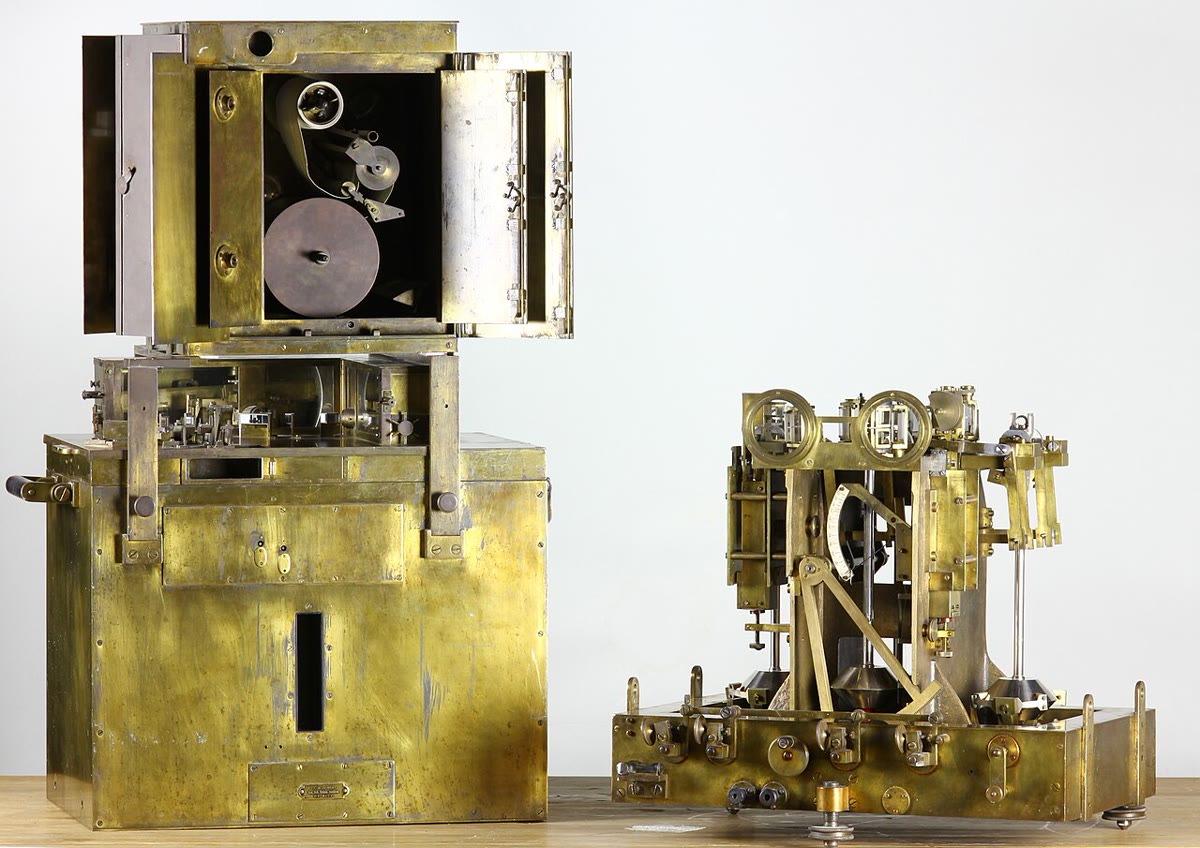
\includegraphics[width=\linewidth]{images/book3/b1-vening-meinesz.jpg}

{\scriptsize Un appareil à pendules de Vening Meinesz (à droite) et son boîtier avec
l'unité d'enregistrement (Broodt, CC BY-SA 4.0).}
\end{minipage}
\end{history}

\section{Le géoïde}

La surface de la mer au repos est une surface de potentiel de pesanteur constant~:
s'il n'en était pas ainsi, l'eau s'écoulerait le long d'elle. C'est la référence
naturelle des hauteurs, et la surface à laquelle les anciens fils à plomb étaient
perpendiculaires.

\begin{definition}[Géoïde~; hauteur du géoïde]\label{def:b1:isostasy-gravity:geoid}
Le \emph{géoïde}\index{geoide@géoïde} est la surface équipotentielle de la pesanteur
de la Terre (gravitation plus effet centrifuge de la rotation) qui coïncide avec
la surface moyenne de la mer au repos sur les océans ouverts, et se prolonge
sous les continents. La \emph{hauteur du géoïde}\index{hauteur du geoide@hauteur du géoïde} $N$ en un
point est la hauteur du géoïde au-dessus de l'ellipsoïde de référence, comptée
négativement là où le géoïde se trouve en dessous.
\end{definition}

Les altitudes au-dessus du niveau de la mer sur les cartes sont des hauteurs
au-dessus du \omterm{def:b1:isostasy-gravity:geoid}{géoïde}~; les hauteurs données par le positionnement par satellite sont
des hauteurs au-dessus de l'ellipsoïde~; les deux diffèrent de
$N$. Le \omterm{def:b1:isostasy-gravity:geoid}{géoïde} s'écarte de l'ellipsoïde de \qty{+85}{m} près de l'Islande et de
\qty{-106}{m} au large du sud de l'Inde, moins de \qty{200}{m} en tout, alors que
le relief de la surface solide s'étend sur environ \qty{20}{km}~: le \omterm{def:b1:isostasy-gravity:geoid}{géoïde} est une
surface bien plus lisse que le sol.
% ledger: nasa:geoid-range, earth:topo

\begin{proposition}[Hauteur du géoïde et anomalie de potentiel]\label{prop:b1:isostasy-gravity:bruns}
Soit $\Phi$ le potentiel de pesanteur de la Terre et $\Phi_n$ le potentiel normal,
celui de la Terre modèle dont la surface, l'ellipsoïde de référence, a le même
potentiel $\Phi_0$ que le \omterm{def:b1:isostasy-gravity:geoid}{géoïde}, tous deux comptés avec le signe de la physique (le
potentiel croît vers le haut et $g = -\nabla\Phi$). Soit $T = \Phi - \Phi_n$ l'anomalie de
potentiel au \omterm{def:b1:isostasy-gravity:geoid}{géoïde}. Au premier ordre,
\[
  N = -\frac{T}{\gamma} .
\]
Les géodésiens, qui comptent le potentiel avec le signe opposé, écrivent le même
résultat $N = T/\gamma$, formule de Bruns.
\end{proposition}

\begin{proof}
Soit $Q$ un point de l'ellipsoïde et $P$ le point du \omterm{def:b1:isostasy-gravity:geoid}{géoïde} sur la
normale passant par $Q$, à la hauteur $N$. Le potentiel normal croît vers le haut
au taux $\gamma$, donc $\Phi_n(P) \approx \Phi_n(Q) + \gamma N = \Phi_0 +
\gamma N$. Comme $P$ est sur le \omterm{def:b1:isostasy-gravity:geoid}{géoïde}, $\Phi(P) = \Phi_0$, c'est-à-dire
$\Phi_n(P) + T = \Phi_0$. D'où $\Phi_0 + \gamma N + T = \Phi_0$ et $N =
-T/\gamma$.
\end{proof}

Un excès de masse sous un point rend le potentiel plus négatif en ce point, donc
$T < 0$ et $N > 0$~: le \omterm{def:b1:isostasy-gravity:geoid}{géoïde} se bombe au-dessus d'un excès de masse et s'enfonce au-dessus
d'un déficit. Les \qty{85}{m} de la bosse près de l'Islande correspondent à une
anomalie de potentiel de $-\qty{85}{m}\times\qty{9.8}{m.s^{-2}} \approx \qty{-830}{J.kg^{-1}}$.
Comme le potentiel décroît en $1/r$ alors que l'attraction décroît en $1/r^2$,
le \omterm{def:b1:isostasy-gravity:geoid}{géoïde} est dominé par de grandes masses profondes, et les \omterm{def:b1:isostasy-gravity:anomalies}{anomalies de pesanteur}
par des masses peu profondes. Une chaîne de montagnes compensée ne relève le \omterm{def:b1:isostasy-gravity:geoid}{géoïde}
que légèrement, parce que son excès de masse et le déficit de sa racine
s'annulent presque~; une charge non compensée le relève bien davantage.

\begin{omfigure}
\begin{tikzpicture}[x=1.15cm, y=1.3cm, font=\scriptsize, >={Stealth[length=4pt]}]
% schematic, not to scale
\fill[omSea!35] (0,0.05) .. controls (1.5,0.25) and (2.5,0.35) .. (3.6,0.45) -- (3.6,-1.2) -- (0,-1.2) -- cycle;
\fill[omLithGranite!40] (3.6,0.45) .. controls (4.5,1.4) and (5.4,1.9) .. (6.4,1.7) .. controls (7.4,1.5) and (8.2,1.2) .. (9,1.0) -- (9,-1.2) -- (3.6,-1.2) -- cycle;
\fill[omLithGabbro!35] (0,-0.7) .. controls (1.2,-0.9) and (2.4,-0.6) .. (3.6,-0.2) -- (3.6,-1.2) -- (0,-1.2) -- cycle;
\draw[thick, blue!70!black] (0,0.05) .. controls (1.5,0.25) and (2.5,0.35) .. (3.6,0.45) .. controls (5,0.75) and (7,0.75) .. (9,0.55);
\draw[thick, black, densely dashed] (0,-0.25) .. controls (3,0.05) and (6,0.15) .. (9,0.1);
\draw (3.6,0.45) .. controls (4.5,1.4) and (5.4,1.9) .. (6.4,1.7) .. controls (7.4,1.5) and (8.2,1.2) .. (9,1.0);
\node[anchor=west, blue!70!black] at (9.05,0.6) {géoïde};
\node[anchor=west] at (9.05,0.1) {ellipsoïde};
\node[anchor=west] at (9.05,1.0) {sol};
\node at (1.4,-0.3) {océan};
\node at (1.6,-1.0) {fond marin};
% heights (curve ordinates computed from the Bezier segments)
\draw[<->] (6.6,0.107) -- (6.6,0.688); \node[anchor=east] at (6.57,0.40) {$N$};
\draw[<->] (7.2,0.674) -- (7.2,1.512); \node[anchor=west] at (7.23,1.09) {$H$};
\draw[<->] (8.2,0.110) -- (8.2,1.224); \node[anchor=east] at (8.17,0.95) {$h_e$};
% the vertical (perpendicular to the geoid) and the ellipsoid normal at x = 2.4 (angle exaggerated)
\draw[->, thick, blue!70!black] (2.4,0.335) -- (2.0,1.3);
\draw[->, thick, black] (2.4,0.335) -- (2.33,1.3);
\node[anchor=south east, blue!70!black] at (2.05,1.3) {verticale (fil à plomb)};
\node[anchor=south west] at (2.3,1.3) {normale à l'ellipsoïde};
\end{tikzpicture}

\par\smallskip{\small Le \omterm{def:b1:isostasy-gravity:geoid}{géoïde} (en bleu), l'ellipsoïde de référence (en tirets) et le
sol (schématique~; écarts énormément exagérés). Sur l'océan le \omterm{def:b1:isostasy-gravity:geoid}{géoïde}
est la surface de la mer au repos~; sous les terres il se prolonge comme une équipotentielle.
La hauteur $H$ sur une carte est mesurée à partir du \omterm{def:b1:isostasy-gravity:geoid}{géoïde}, la hauteur $h_e$ donnée
par le positionnement par satellite à partir de l'ellipsoïde, et $h_e = H + N$. Un fil à plomb est
perpendiculaire au \omterm{def:b1:isostasy-gravity:geoid}{géoïde}, non à l'ellipsoïde~: l'angle entre eux
(exagéré ici) est la déviation de la verticale qui tourmentait les
arpenteurs de l'Inde.}
\label{fig:b1:isostasy-gravity:geoid}
\end{omfigure}

Les déviations sont petites~: tout le désaccord qui tourmentait les arpenteurs
de l'Inde était d'environ cinq secondes d'arc. Sur les océans le \omterm{def:b1:isostasy-gravity:geoid}{géoïde} est visible.
Depuis 1978, des altimètres radar sur satellites ont chronométré des impulsions micro-ondes
réfléchies par la surface de la mer pour mesurer sa hauteur. Une fois les marées, les
vagues et les courants moyennés, la surface de la mer se tient plus haut au-dessus des monts
sous-marins et des dorsales et plus bas au-dessus des fosses et des plaines abyssales, et ces
bosses (l'\cref{exo:b1:isostasy-gravity:11}
en estime une) cartographient le relief du plancher océanique profond là où aucun navire n'a
sondé. Le satellite GOCE, de 2009 à 2013, a volé à environ \qty{260}{km}
et mesuré le champ de pesanteur depuis l'orbite, visant le \omterm{def:b1:isostasy-gravity:geoid}{géoïde} à 1 à
\qty{2}{cm} et les \omterm{def:b1:isostasy-gravity:anomalies}{anomalies de pesanteur} à environ \qty{1}{\milli\gal}, avec une
résolution meilleure que \qty{100}{km}.
% ledger: pratt:himalaya, jpl:seasat, esa:goce

\subsection*{L'isostasie en mouvement}

L'\omterm{def:b1:isostasy-gravity:isostasy}{isostasie} s'atteint par un écoulement, et un écoulement prend du temps. Au maximum
de la dernière glaciation, il y a environ \num{20000} ans, une calotte de glace épaisse
d'environ \qty{3}{km} recouvrait la Scandinavie.
La glace est environ neuf dixièmes aussi dense que l'eau, donc avec un \omterm{def:b1:layered-earth:layers}{manteau} de
\qty{3300}{kg.m^{-3}}, l'enfoncement isostatique complet sous une telle calotte est
$\qty{3000}{m}\times900/3300 \approx \qty{820}{m}$. La glace a disparu, et la
terre remonte encore~: le positionnement par satellite mesure jusqu'à environ
\qty{10}{mm.an^{-1}} de soulèvement dans le nord de la Suède, à l'ouest du golfe de Botnie,
aujourd'hui. La
vitesse à laquelle une dépression se relâche mesure la viscosité du \omterm{def:b1:layered-earth:layers}{manteau} en dessous,
sujet du livre~5~; l'\cref{exo:b1:isostasy-gravity:12} montre comment.
% ledger: kierulf:fennoscandia, usgs:ice-density

\section{Exercices}

\begin{exercise}[$\star$]\label{exo:b1:isostasy-gravity:1}
(a) Convertir une \omterm{def:b1:isostasy-gravity:anomalies}{anomalie de Bouguer} de \qty{-150}{\milli\gal} en \unit{m.s^{-2}},
et l'exprimer comme une fraction de $g = \qty{9.81}{m.s^{-2}}$. (b) La même chose pour
\qty{1}{\milli\gal}, la précision visée pour les \omterm{def:b1:isostasy-gravity:anomalies}{anomalies de pesanteur} issues de
GOCE, et pour \qty{1}{\micro\gal}.
% ledger: esa:goce, nist:gal
\end{exercise}

\begin{exercise}[$\star$]\label{exo:b1:isostasy-gravity:2}
(a) Calculer la \omterm{def:b1:isostasy-gravity:normal-gravity}{pesanteur normale} à l'équateur, à \ang{45} et aux pôles avec
la formule du chapitre. (b) Donner la différence équateur--pôle en
milligals. (c) L'accélération centrifuge à l'équateur est de
\qty{3392}{\milli\gal}. Quelle fraction de la différence la rotation
explique-t-elle directement~?
% ledger: moritz:grs80
\end{exercise}

\begin{exercise}[$\star$]\label{exo:b1:isostasy-gravity:3}
Un plateau se dresse à \qty{3}{km} au-dessus du niveau de la mer. Avec une \omterm{def:b1:layered-earth:layers}{croûte} de masse
volumique \qty{2800}{kg.m^{-3}} et un \omterm{def:b1:layered-earth:layers}{manteau} de \qty{3300}{kg.m^{-3}}, calculer sa racine
d'Airy et l'épaississement de sa \omterm{def:b1:layered-earth:layers}{croûte}.
\end{exercise}

\begin{exercise}[$\star$]\label{exo:b1:isostasy-gravity:4}
(a) De combien faut-il élever un gravimètre pour que sa lecture diminue de
\qty{1}{\milli\gal}~? Utiliser \qty{0.3086}{\milli\gal.m^{-1}}. (b) Un levé vise des
anomalies à \qty{0.01}{\milli\gal}. Avec quelle exactitude les hauteurs des stations
doivent-elles être connues~?
\end{exercise}

\begin{exercise}[$\star\star$]\label{exo:b1:isostasy-gravity:5}
Dans le modèle de Pratt avec $D = \qty{100}{km}$ et $\rho_0 = \qty{2700}{kg.m^{-3}}$,
(a) calculer la masse volumique des colonnes hautes de 1, 3 et \qty{5}{km}~;
(b) calculer la masse volumique d'une colonne sous \qty{4}{km} d'eau de mer de masse volumique
\qty{1030}{kg.m^{-3}}. (c) Pourquoi le modèle de Pratt convient-il mieux au plancher
océanique qu'aux continents~?
\end{exercise}

\begin{exercise}[$\star\star$]\label{exo:b1:isostasy-gravity:6}
Deux stations se trouvent à la \omterm{def:b1:spherical-astronomy:geographic}{latitude} \ang{48}, où la \omterm{def:b1:isostasy-gravity:normal-gravity}{pesanteur normale} est de
\qty{9.808911}{m.s^{-2}}. La station 1, à \qty{350}{m} au-dessus du niveau de la mer, lit
\qty{9.807751}{m.s^{-2}}~; la station 2, à \qty{1850}{m}, lit
\qty{9.803552}{m.s^{-2}}. (a) Calculer les \omterm{def:b1:isostasy-gravity:anomalies}{anomalies à l'air libre} et de Bouguer des
deux, avec la masse volumique de Bouguer standard. (b) Que suggèrent les anomalies de la
station 2 sur les montagnes qui l'entourent~?
\end{exercise}

\begin{exercise}[$\star\star$]\label{exo:b1:isostasy-gravity:7}
(a) En suivant la démonstration de la \cref{prop:b1:isostasy-gravity:slab}, montrer
qu'un disque horizontal de rayon $a$, d'épaisseur $h$ et de masse volumique $\rho$ attire un point
sur son axe, à une distance $z \gg h$ au-dessus de lui, avec $2\pi G\rho h\,\bigl(1 -
z/\sqrt{z^2 + a^2}\bigr)$. (b) Quel rayon donne \qty{90}{\percent} de la valeur de
la plaque à $z = \qty{1}{km}$~? (c) Qu'est-ce que cela dit de l'aire de terrain
qui compte pour la \omterm{def:b1:isostasy-gravity:anomalies}{correction de Bouguer}~?
\end{exercise}

\begin{exercise}[$\star\star$]\label{exo:b1:isostasy-gravity:8}
Dans le modèle d'Airy avec une \omterm{def:b1:layered-earth:layers}{croûte} de \qty{2800}{kg.m^{-3}}, épaisse de \qty{35}{km} au niveau de la
mer, sur un \omterm{def:b1:layered-earth:layers}{manteau} de \qty{3300}{kg.m^{-3}}, (a) calculer l'anti-racine et
l'épaisseur de la \omterm{def:b1:layered-earth:layers}{croûte} sous \qty{4}{km} d'eau de mer de masse volumique \qty{1030}{kg.m^{-3}}.
(b) La \omterm{def:b1:layered-earth:layers}{croûte} océanique fait en fait environ \qty{5}{km} d'épaisseur. Que montre la
différence~? % ledger: usgs:crust-thickness
\end{exercise}

\begin{exercise}[$\star\star$]\label{exo:b1:isostasy-gravity:9}
Dans le récit d'ouverture, le désaccord sur la différence de \omterm{def:b1:spherical-astronomy:geographic}{latitude}
entre Kaliana et Kalianpur était de \qty{5.236}{''}, alors que l'attraction de
l'Himalaya calculée par Pratt aurait dû produire \qty{15.885}{''}. (a) Convertir
les deux angles en radians. (b) Une accélération horizontale $a_h$ incline un fil à plomb de
l'angle $a_h/g$. À quelle différence d'attraction horizontale entre les deux
stations chaque angle correspond-il, en milligals, avec
$g = \qty{9.79}{m.s^{-2}}$~? (c) Quelle fraction de l'attraction des
montagnes visibles la compensation a-t-elle annulée~?
% ledger: pratt:himalaya
\end{exercise}

\begin{exercise}[$\star\star\star$]\label{exo:b1:isostasy-gravity:10}
Un dôme de sel est modélisé par une sphère de rayon \qty{2}{km}, de centre à
\qty{4}{km} de profondeur, de masse volumique inférieure de \qty{200}{kg.m^{-3}} à celle des roches
qui l'entourent. (a) Montrer qu'une sphère enfouie de masse anormale $M$ à la profondeur $z$
donne, à la distance horizontale $x$, l'anomalie $GMz/(x^2 + z^2)^{3/2}$.
(b) Calculer l'anomalie à l'aplomb de son centre. (c) À quelle distance est-elle tombée
à la moitié de son maximum~? (d) Comment pourrait-on lire la profondeur d'une sphère sur un profil
mesuré~?
\end{exercise}

\begin{exercise}[$\star\star\star$]\label{exo:b1:isostasy-gravity:11}
Un mont sous-marin est un cône haut de \qty{3}{km} dont la base a un rayon de \qty{15}{km},
posé sur un plancher marin profond de \qty{5}{km}. Sa roche a une masse volumique de
\qty{2800}{kg.m^{-3}}, l'eau de mer \qty{1030}{kg.m^{-3}}. (a) Calculer son excès de
masse par rapport à l'eau qu'il déplace. (b) Le traiter comme une masse ponctuelle en son centre de
masse, au quart de sa hauteur au-dessus de la base, et utiliser
la \cref{prop:b1:isostasy-gravity:bruns} avec $\gamma = \qty{9.81}{m.s^{-2}}$ pour
estimer la hauteur de la bosse de la surface de la mer au-dessus de lui. (c) La masse
ponctuelle sur- ou sous-estime-t-elle la bosse~? (d) Si le mont sous-marin était entièrement
compensé par une racine, comment la bosse changerait-elle~?
\end{exercise}

\begin{exercise}[$\star\star\star$]\label{exo:b1:isostasy-gravity:12}
Modéliser le relèvement de la Scandinavie après la glace~: supposons que la glace ait disparu
brusquement il y a \num{10000} ans, laissant une dépression de \qty{818}{m} qui a
depuis diminué comme $w(t) = w_0\,e^{-t/\tau}$. (a) Montrer que la vitesse de soulèvement est
$w/\tau$. (b) Avec $\tau = \num{4000}$ ans, calculer la dépression restante
et la vitesse de soulèvement aujourd'hui, et comparer la vitesse à la valeur mesurée de
\qty{10}{mm.an^{-1}}. (c) Montrer que $\tau = \num{3100}$ ans et
$\tau = \num{68000}$ ans donnent tous deux environ \qty{10}{mm.an^{-1}} aujourd'hui. Quelle
dépression restante chacun implique-t-il, et comment un levé gravimétrique pourrait-il départager
les deux~? (d) Quelle propriété du \omterm{def:b1:layered-earth:layers}{manteau} $\tau$ mesure-t-il~?
% ledger: kierulf:fennoscandia
\end{exercise}

\section{Problème~: La racine d'une chaîne de montagnes}

\begin{problem}[{Problème du week-end --- la racine d'un plateau, Airy contre Pratt,
la pesanteur au-dessus de lui, et ce que l'érosion lui fait}]
\label{pb:b1:isostasy-gravity:1}
% values: calc/ch11.py (invented plateau; normal gravity formula of the chapter)
% ledger: moritz:grs80, usgs73:reduction
Un large plateau, de plusieurs centaines de kilomètres de large, se dresse à \qty{4}{km} au-dessus d'une
plaine au niveau de la mer dont la \omterm{def:b1:layered-earth:layers}{croûte} fait \qty{35}{km} d'épaisseur. Prendre
$\rho_c = \qty{2700}{kg.m^{-3}}$ pour la \omterm{def:b1:layered-earth:layers}{croûte}, $\rho_m = \qty{3300}{kg.m^{-3}}$
pour le \omterm{def:b1:layered-earth:layers}{manteau}, $g = \qty{9.81}{m.s^{-2}}$, et
$2\pi G = \qty{0.0419}{\milli\gal}$ par mètre et par \qty{1000}{kg.m^{-3}}.

\medskip
\noindent\textbf{Partie I --- Le plateau d'Airy.}
\begin{enumerate}
  \item Calculer la racine d'Airy du plateau.
  \item En déduire l'épaisseur de sa \omterm{def:b1:layered-earth:layers}{croûte} et la profondeur de son \omterm{def:b1:layered-earth:discontinuity}{Moho} sous le niveau de
        la mer.
  \item Prendre la \omterm{def:b1:isostasy-gravity:isostasy}{profondeur de compensation} à \qty{60}{km} sous le niveau de la mer. Calculer la
        masse par mètre carré au-dessus d'elle dans la colonne du plateau et dans la colonne
        de la plaine.
  \item Calculer la pression à \qty{60}{km} de profondeur.
  \item Pourquoi la racine est-elle 4.5 fois la hauteur~? Quel serait le rapport avec une
        \omterm{def:b1:layered-earth:layers}{croûte} de \qty{2900}{kg.m^{-3}}~?
  \item Que montrerait un levé de sismique réfraction à travers le bord du plateau
        si le modèle d'Airy est valable~?
\end{enumerate}

\noindent\textbf{Partie II --- Le plateau de Pratt.}
Supposons maintenant plutôt une \omterm{def:b1:isostasy-gravity:isostasy}{profondeur de compensation} $D = \qty{100}{km}$ sous le niveau de la mer et
une colonne de plaine de masse volumique uniforme \qty{2700}{kg.m^{-3}}.
\begin{enumerate}[resume]
  \item Calculer la masse volumique de la colonne du plateau.
  \item Vérifier que les deux colonnes ont la même masse par mètre carré au-dessus de
        $D$.
  \item De combien, en pour cent, la colonne du plateau doit-elle être plus légère~?
  \item Si cette différence de masse volumique était due à la seule chaleur, avec un
        coefficient de dilatation thermique de \qty{3e-5}{K^{-1}}, de combien la colonne du
        plateau devrait-elle être plus chaude en moyenne~? Est-ce plausible~?
  \item Où est le \omterm{def:b1:layered-earth:discontinuity}{Moho} sous le plateau dans le modèle de Pratt~?
  \item Un levé de réfraction trouve le \omterm{def:b1:layered-earth:discontinuity}{Moho} à \qty{52}{km} sous le plateau.
        Quel modèle convient~?
\end{enumerate}

\noindent\textbf{Partie III --- La pesanteur au centre.}
\begin{enumerate}[resume]
  \item Calculer la \omterm{def:b1:isostasy-gravity:anomalies}{correction de Bouguer} pour une station sur le plateau.
  \item Prédire les \omterm{def:b1:isostasy-gravity:anomalies}{anomalies à l'air libre} et de Bouguer au centre si le plateau
        n'était pas compensé.
  \item Les prédire pour le plateau d'Airy, et vérifier l'\omterm{def:b1:isostasy-gravity:anomalies}{anomalie de Bouguer} avec
        la masse manquante de la racine.
  \item Une station au centre du plateau, à la \omterm{def:b1:spherical-astronomy:geographic}{latitude} \ang{30} et à
        \qty{4000}{m}, lit \qty{9.781085}{m.s^{-2}}. Calculer la \omterm{def:b1:isostasy-gravity:normal-gravity}{pesanteur normale}
        à \ang{30}, puis les \omterm{def:b1:isostasy-gravity:anomalies}{anomalies à l'air libre} et de Bouguer.
  \item Quelle fraction du plateau est compensée~?
  \item L'\omterm{def:b1:isostasy-gravity:anomalies}{anomalie de Bouguer} au centre serait-elle différente si le plateau
        était compensé à la manière de Pratt~? Expliquer.
  \item Esquisser l'\omterm{def:b1:isostasy-gravity:anomalies}{anomalie à l'air libre} le long d'un profil à travers un bord du
        plateau, et expliquer sa forme.
\end{enumerate}

\noindent\textbf{Partie IV --- L'érosion.}
Des rivières enlèvent une couche épaisse de \qty{1}{km} sur toute la surface du plateau,
assez lentement pour que l'\omterm{def:b1:isostasy-gravity:isostasy}{isostasie} suive.
\begin{enumerate}[resume]
  \item Quelle est la nouvelle épaisseur de la \omterm{def:b1:layered-earth:layers}{croûte}, et sa nouvelle racine d'Airy~?
  \item Quelle est la nouvelle altitude du plateau~?
  \item De combien la roche qui est maintenant à la surface est-elle remontée~?
  \item Quelle quantité de roche faut-il éroder en tout pour ramener le plateau au niveau de la
        mer~? Qu'est-ce que cela dit des roches que l'on voit dans les vieilles chaînes de montagnes~?
  \item De combien la surface du plateau s'abaisse-t-elle pour chaque
        kilomètre de roche érodé~?
\end{enumerate}
\end{problem}
